\section{Experimental setup}\label{sec:setup}

The experiment is staged so that vector construction, operating-point selection, and final evaluation use separate data. We first build each steering direction, then choose a setting that improves validation behavior without sacrificing coherence, and only then run the projection and its controls on the held-out test set.

\paragraph{Model and precision.}
All experiments use Llama-3-8B-Instruct \citep{grattafiori2024llama3} ($L=32$, $d=4096$, $V=128{,}256$, RMSNorm) in bfloat16. Projections and certificates are computed in float64.

\paragraph{Staged data split.}
TruthfulQA \citep{lin2022truthfulqa} supplies the multiple-choice behavioral benchmark of 817 questions. A seeded shuffle assigns 120 questions to a validation slice used only for operating-point selection, 200 to the construction of mass-mean statements, and the remaining 497 to the held-out test slice on which every headline number is computed.

The CAA vector uses a separate 400-instruction Alpaca pool \citep{taori2023alpaca}. Of these instructions, 256 are rendered under honest and deceptive system prompts to construct the vector, a disjoint block of 96 supplies held-out fluency text for the coherence gate, and the remaining 48 supply the statistical token set. These statistical sets are deliberately data-driven rather than semantic: they admit punctuation and fragment tokens whose first-position logits shift under the system-prompt contrast, and serve as a control construction rather than a curated lexicon. The 256 construction instructions, re-rendered as plain chat prompts without a system prompt, also form the effective-unembedding calibration set; $J_{\gamma}$ is averaged over their pre-norm final-layer residuals at the last prompt position. Vector-construction and evaluation data share no prompts.

\paragraph{Steering-vector families.}
We compare two forms of supervision under the same unembedding apparatus. The \emph{CAA} vector \citep{rimsky2024caa} is the difference of mean final-token residuals between honest- and deceptive-prompted renderings, computed per layer. The \emph{mass-mean} vector \citep{marks2024geometry} is the difference of mean residuals between true and false \texttt{Q:/A:} statements assembled from the 200 reserved TruthfulQA questions, computed at the same candidate layers. Each family is analyzed at its own operating point with its own projections; the unembedding apparatus is shared.

\paragraph{Coherence-gated operating points.}
Before decomposing an effect, we first establish that there is a coherent effect to decompose. For each family, we sweep layers $\ell \in \{12, 14\}$ and six strengths $\alpha$ from $0.5$ to $4$. Every setting receives two validation measurements: its MC2 improvement and its ratio of held-out per-token perplexity to baseline on the 96 reserved Alpaca instructions. We call a setting \emph{coherent} when that ratio is at most $1.5$, then select the coherent setting with the largest validation MC2 gain.

The gate is necessary because teacher-forced multiple-choice scores are largely insensitive to generation collapse. A sufficiently large $\alpha$ can raise MC2 while degrading free generation to incoherent output (Section~\ref{sec:results}), so maximizing MC2 alone selects precisely such a regime. The gate instead selects $(\ell^{*}{=}12, \alpha^{*}{=}3)$ for CAA and $(\ell^{*}{=}12, \alpha^{*}{=}4)$ for mass-mean; Figure~\ref{fig:calibration} shows the complete grid. The conclusion does not depend on the exact threshold. The mass-mean operating point remains $(\ell^{*}{=}12, \alpha^{*}{=}4)$ for every gate in $[1.2, 2.0]$, because it maximizes validation gain among coherent settings throughout that range. CAA's selected point changes with the threshold, but its $\rho$ remains uninterpretable at every such point because its denominator is statistically zero.

\begin{figure}[t]
\centering
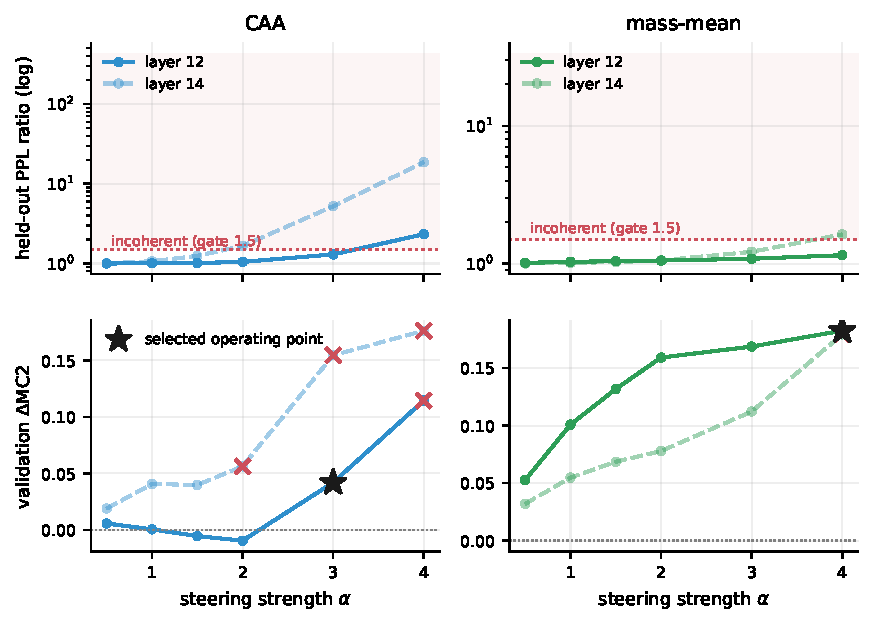
\includegraphics[width=0.92\textwidth]{../figures/calibration.pdf}
\caption{Coherence calibration: held-out perplexity ratio against steering strength $\alpha$ for each candidate layer, with the gate at $1.5$ (dashed). CAA crosses the gate between $\alpha{=}3$ and $\alpha{=}4$ at layer 12 and earlier at layer 14; the mass-mean vector stays coherent across nearly the whole grid.}
\label{fig:calibration}
\end{figure}

\paragraph{Primary evaluation.}
TruthfulQA MC follows the original scoring rule. MC1 is the accuracy of the highest-scoring answer choice; MC2 is the normalized probability mass on all true choices, where each choice is scored by its total log-probability. We score choices zero-shot under the prompt \texttt{Q: \{question\}\textbackslash nA:}, not behind the original six-example QA primer. Because every condition uses the same prompt, all reported contrasts are internal, and the absolute scores are not directly comparable with primer-based results in the literature. Prompt and continuation are tokenized separately and concatenated at the id level; this matches tokenizing the joined string for all \BpePairs{} prompt--choice pairs in the benchmark (\BpeMismatches{} mismatches). The intervention is active at every token position.

The primary causal contrast compares each family's $\vdec$ with its aligned-64 projection $\vperp$ on the 497 held-out questions, against a shared unsteered baseline. We then test the interpretation from several directions: aligned-$k$ projections for $k \in \{16, 64, 256, 1024\}$ trace rank sensitivity; curated and statistical projections vary the token-set construction; $\vpar$ (aligned-64) tests the readout-aligned component in isolation; a norm-matched $\vperp$ separates direction from magnitude; and random 64-dimensional projections under three seeds test whether the aligned subspace is special. Every condition within a family uses that family's $(\ell^{*}, \alpha^{*})$.

At the answer position, we also record every token logit in the union of the curated, spillover, statistical, and aligned-64 sets. The stem-disjoint spillover sets are synonym lexicons excluded from every projection. These logged values yield the honest-shift $\eta$ and spillover readouts without additional forward passes.

\paragraph{Out-of-distribution and process probes.}
After the headline contrast, we ask whether the result survives a change in phrasing and where any vocabulary effect re-emerges. The unsteered model paraphrases the first 150 test questions by greedy decoding under a meaning-preserving instruction. We rescore those questions under baseline, $\vdec$, and aligned-64 $\vperp$ for each family, producing the OOD depth ratio $\rho_{\mathrm{OOD}}$. The spillover readout evaluates $\eta$ on stem-disjoint synonym sets that were never projected out, while a logit-lens trajectory \citep{nostalgebraist2020logitlens} follows the curated-$T$ readout across layers under $\vdec$, $\vperp$, and $\vpar$ to localize where the honest-shift re-emerges.

\paragraph{Reproducibility and numerical checks.}
The pipeline is staged and checkpointed with fixed seeds; all code, token lists, certificates, and the formal proof are in the repository. The zero-direct-effect certificates $\max_t |(A\vperp)_t|$ are at most \CertWorst{} logits across every family and token set---machine precision in float64---against pre-projection direct effects of up to \CertPre{} logits per unit $\alpha$. Forward passes run in bfloat16 without enforced kernel determinism, so individual per-question scores can shift at the third decimal across reruns; every reported interval is orders of magnitude wider. With the vector, gate, and controls fixed before final evaluation, we first show why benchmark-only selection fails and then apply the decomposition to the two steering families.
